\documentclass[12pt, titlepage]{article}
\usepackage[utf8]{inputenc}
\usepackage{amsmath,amsthm,amsfonts,amssymb,amscd}
\usepackage{multirow,booktabs}
\usepackage[table]{xcolor}
\usepackage{fullpage}
\usepackage{lastpage}
\usepackage{enumitem}
\usepackage{fancyhdr}
\usepackage{mathrsfs}
\usepackage{wrapfig}
\usepackage{setspace}
\usepackage{calc}
\usepackage{multicol}
\usepackage{cancel}
\usepackage[retainorgcmds]{IEEEtrantools}
\usepackage[margin=3cm]{geometry}
\usepackage{amsmath}
\newlength{\tabcont}
\setlength{\parindent}{0.0in}
\setlength{\parskip}{0.05in}
\usepackage{empheq}
\usepackage{framed}
\usepackage[most]{tcolorbox}
\usepackage{xcolor}
\colorlet{shadecolor}{orange!15}
\parindent 0in
\parskip 12pt
\geometry{margin=1in, headsep=0.25in}
\theoremstyle{definition}
\newtheorem{defn}{Definition}
\newtheorem{reg}{Rule}
\newtheorem{exer}{Exercise}
\newtheorem{note}{Note}

\usepackage[superscript,biblabel]{cite}
\usepackage{hyperref}
\hypersetup{colorlinks,linkcolor={blue},citecolor={blue},urlcolor={orange}}

\usepackage{graphicx}
% Path relative to the main .tex file
\graphicspath{ {./images/} }

\title{\textbf{Practical integrator using operational amplifier}}
\author{
  Russel Shawn Dsouza\\
  171EC143
  \and
  Sathvik S Prabhu\\
  171EC146
}
\date{13 November 2019}

% Vertical spacing for aligned equations
\setlength{\jot}{10pt}
% https://tex.stackexchange.com/a/42728
\newcommand\numberthis{\addtocounter{equation}{1}\tag{\theequation}}

\begin{document}
  % TODO Add NITK logo
  % TODO Add 'AIC Report' and date
  \maketitle
  \thispagestyle{empty}

  \newpage
  \tableofcontents
  \thispagestyle{empty}

  \newpage
  \setcounter{page}{1}
  \section{Aim}
  To design, implement and test a $\mu$A741-based voltage integrator.


  \section*{Components required}
    \begin{itemize}
      \item $\mu$A741 op-amp
      \item Resistors R = 120k$\Omega$, 3.3k$\Omega$, 4.7k$\Omega$
      \item Capacitor C = 0.01 $\mu$F
      \item Signal generator
      \item Digital Storage Oscilloscope
      \item Breadboard
      \item Jumper wires
    \end{itemize}


  \newpage
  \section{Circuit diagram}
    \begin{figure}[h]
      \centering
      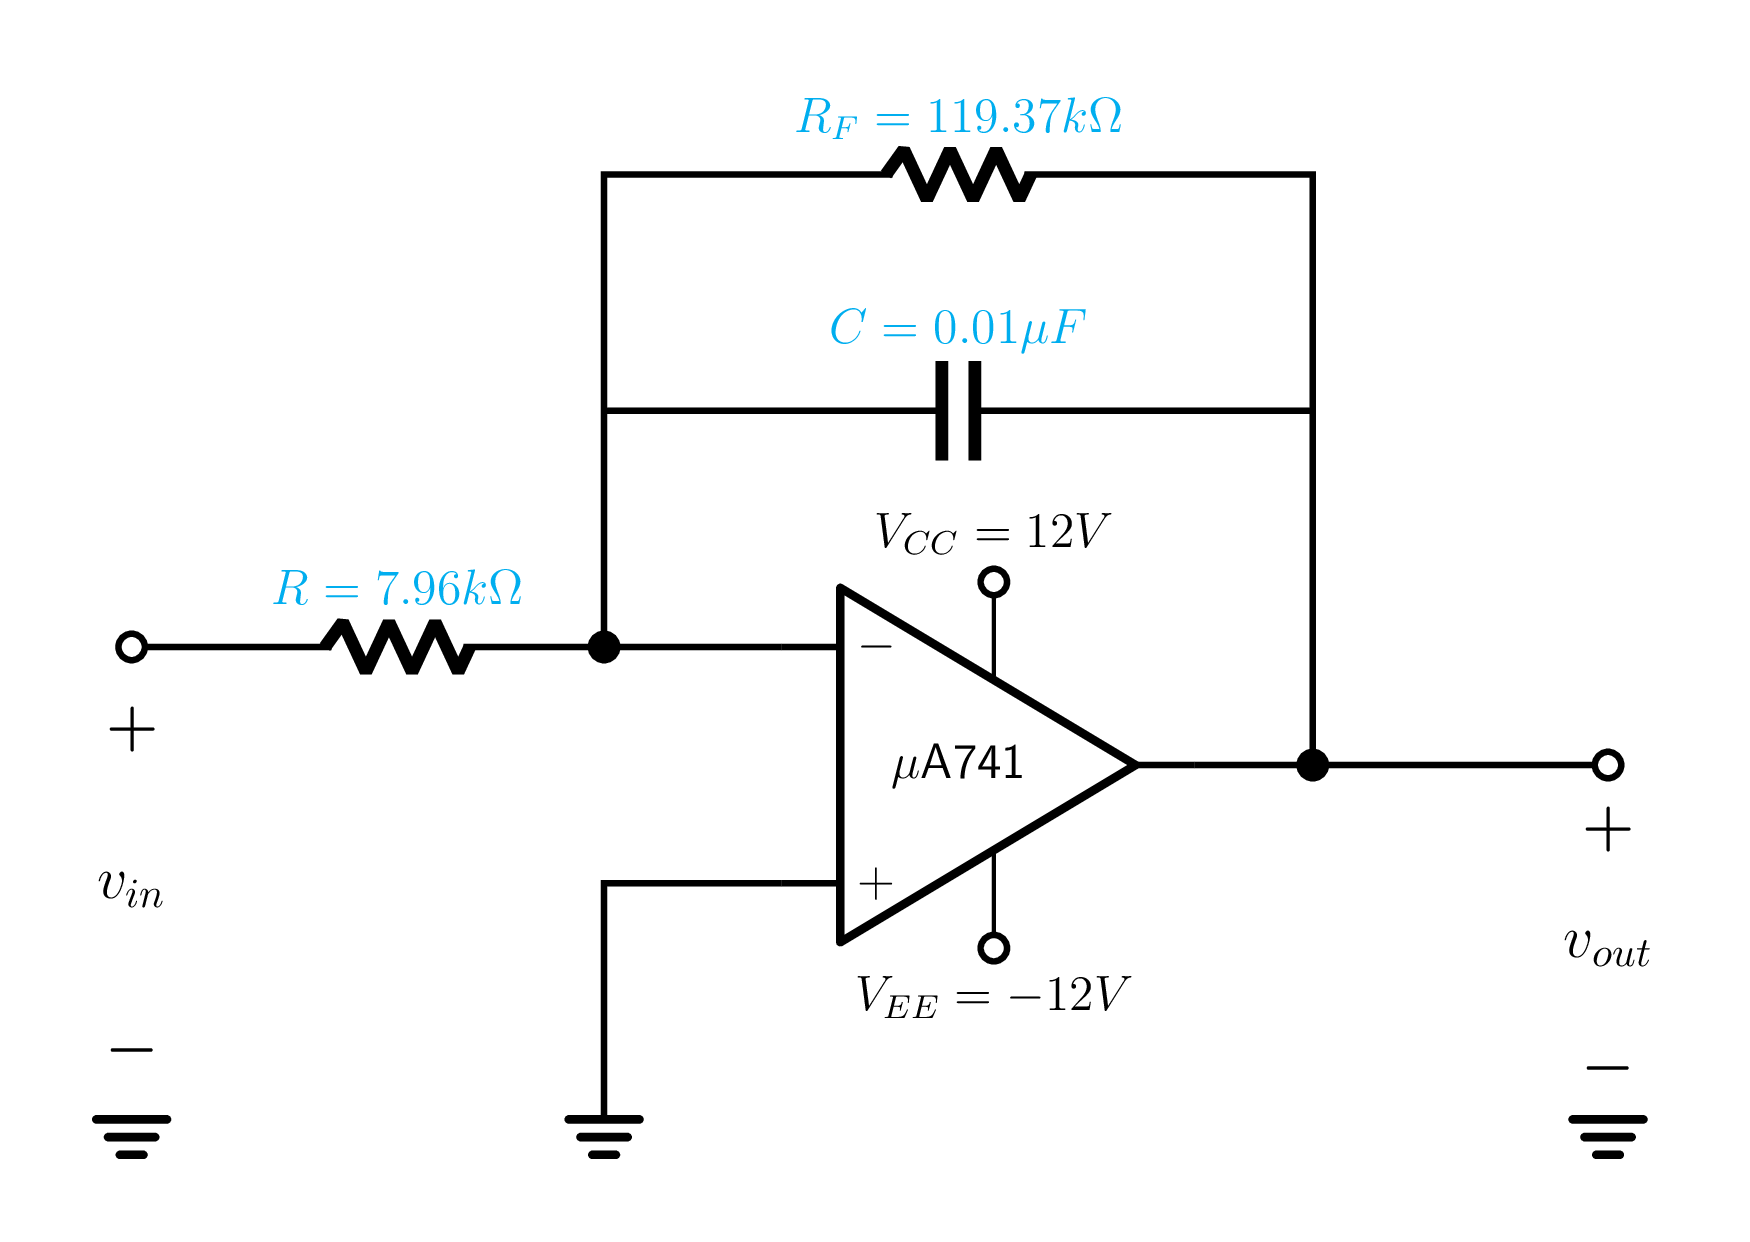
\includegraphics[scale=0.25]{images/designed_practical_integrator.png}
      \caption{Final design of the practical integrator}
      \label{fig:designed_practical_integrator}
    \end{figure}

  \newpage
  \section{Theory}
    %===Basics of op-amp integrator===
    The operational amplifier based integrator performs the mathematical operation of integration with respect to time, i.e. its output is proportional to the input voltage integrated over time.
    The integrator circuit is mostly used in analog computers, analog-to-digital converters and wave-shaping circuits such as charge amplifiers.

    The response of an op-amp circuit with feedback reflects the characteristics of the feedback elements. Thus, in order to achieve integration, the feedback network is constructed using a capacitor.

    %===Ideal op-amp integrator===
    An operational amplifier based integrator can ideally be constructed as shown in figure \ref{fig:theoretical_ideal_integrator}.

    \begin{figure}[h]
      \centering
      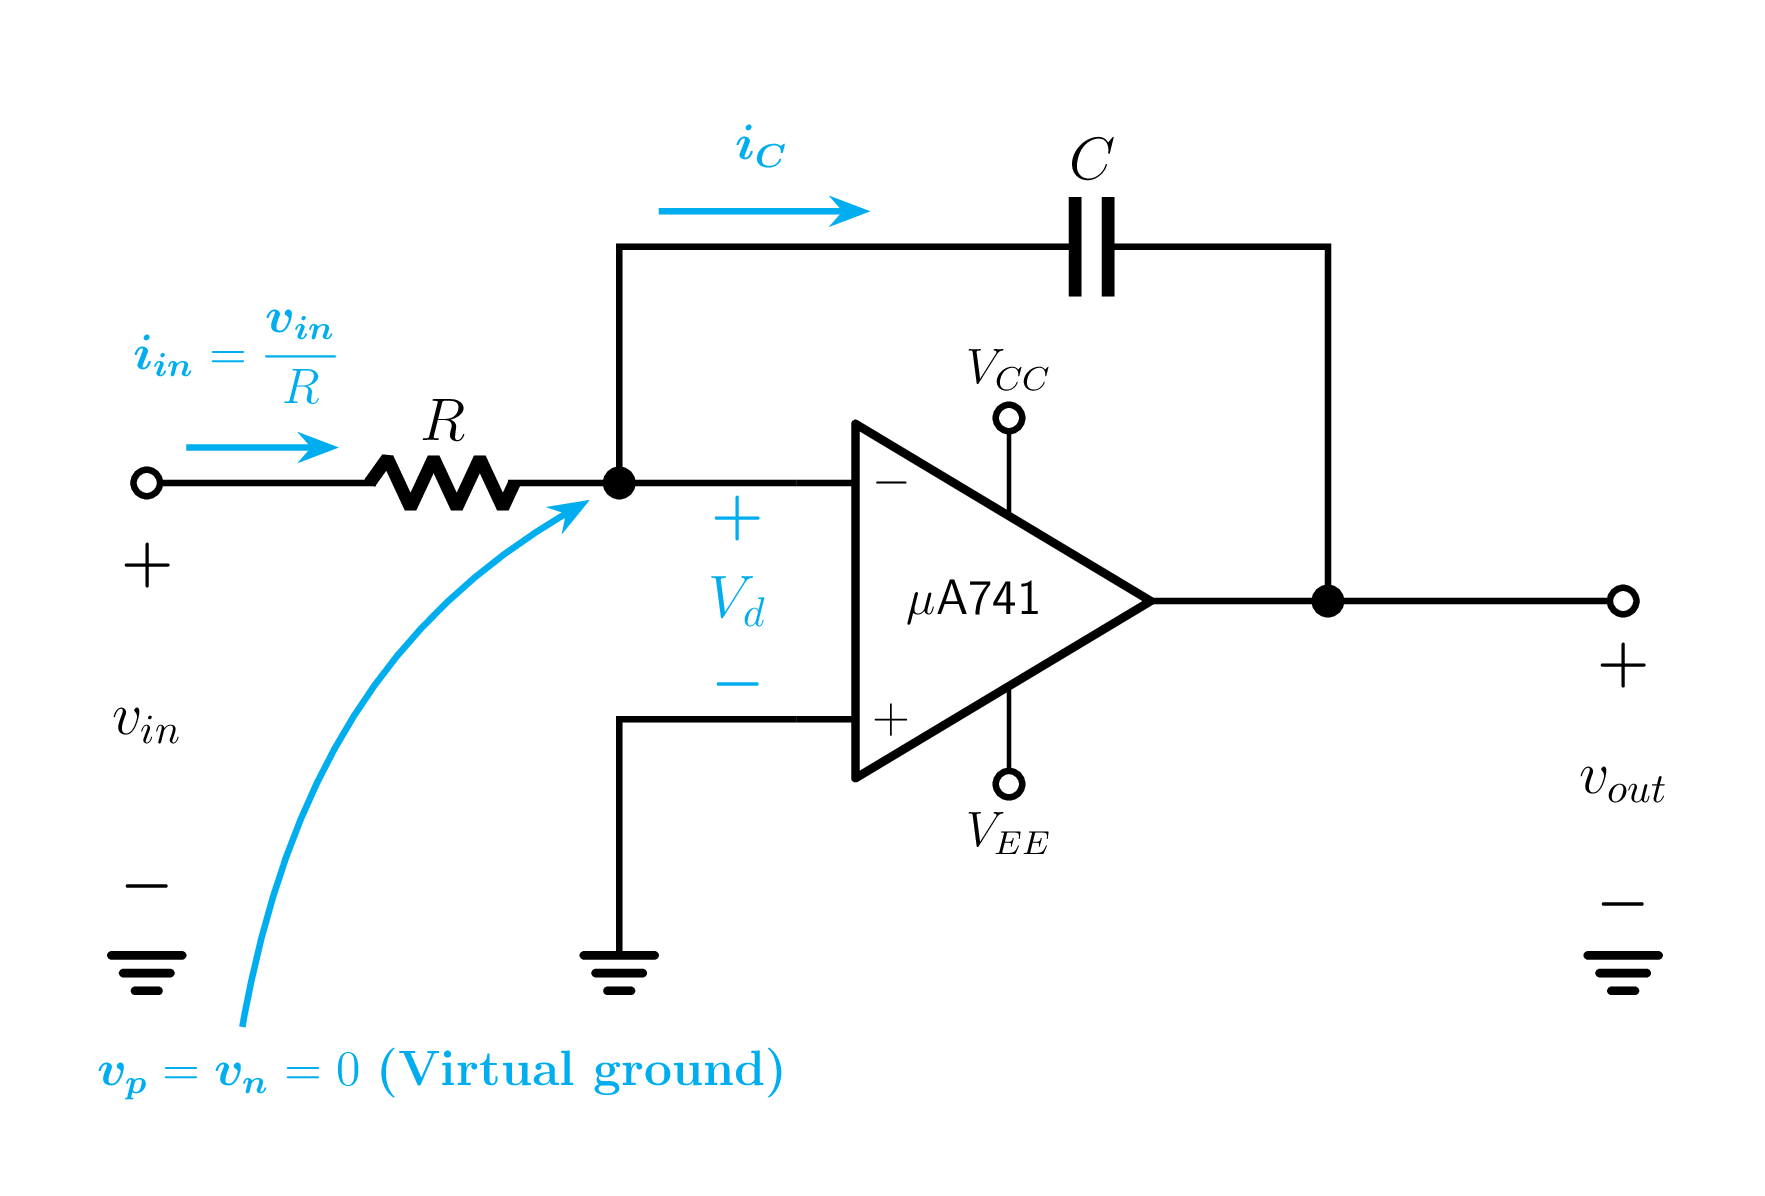
\includegraphics[scale=0.25]{images/ideal_integrator.png}
      \caption{Ideal op-amp based integrator}
      \label{fig:theoretical_ideal_integrator}
    \end{figure}

    The circuit can be analysed by applying Kirchhoff's current law at the node $V_n$, keeping ideal op-amp behaviour in mind.
    \begin{equation}\label{eq:ideal_kcl_vn}
      i_{in} = I_C = \cfrac{V_{in}}{R}
    \end{equation}

    The relationship between between the capacitor's voltage and current is modelled as:
    \begin{equation}\label{eq:ideal_i-v_cap}
      I_C = C\cfrac{dV_C}{dt}
    \end{equation}

    Substituting eq. \ref{eq:ideal_kcl_vn} in eq. \ref{eq:ideal_i-v_cap}:
    \begin{align*}
      \cfrac{v_{in} - 0}{R} &= C\cfrac{d(0 - v_{out})}{dt}
      \implies \cfrac{v_{in}}{R} = -C\cfrac{dv_{out}}{dt}
    \end{align*}

    Integrating both sides with respect to time:
    \begin{align*}
      \int_0^t {\cfrac{v_{in}}{R}} &= - \int_0^t {\cfrac{dv_{out}}{dt}dt} \\
      v_{out} &= -\cfrac{1}{RC} \int_0^t {\cfrac{dv_{out}}{dt}}
    \end{align*}
    Thus the output of the circuit shown in figure \ref{fig:theoretical_ideal_integrator} is the inverted, integrated input with a gain of $\cfrac{1}{RC}$.

    %===Limitations of ideal integrator===
    The ideal integrator suffers from two main limitations. One comes from the fact that the output volatage of the op-amp cannot exceed the supply voltage.
    The output of the integrator is inversely proportional to the time constant $\tau = RC$.
    The larger the time constant $\tau$ ,the longer it takes to saturate the integrator.
    The second limitation is a consequence of the offset voltage present even for zero input.
    It may be only a few milivolts, but this gets integrated over time and it eventually drives the op-amp to saturation.

    %===Practical op-amp integrator===
    One can overcome the limitations of an ideal integrator by adding a resistor $R_{f}$ in parallel with capacitor $C$ as shown in figure \ref{fig:theoretical_practical_integrator}. $R_{f}$ prevents the op-amp from going into open loop configuration at low frequencies.

    \begin{figure}[h]
      \centering
      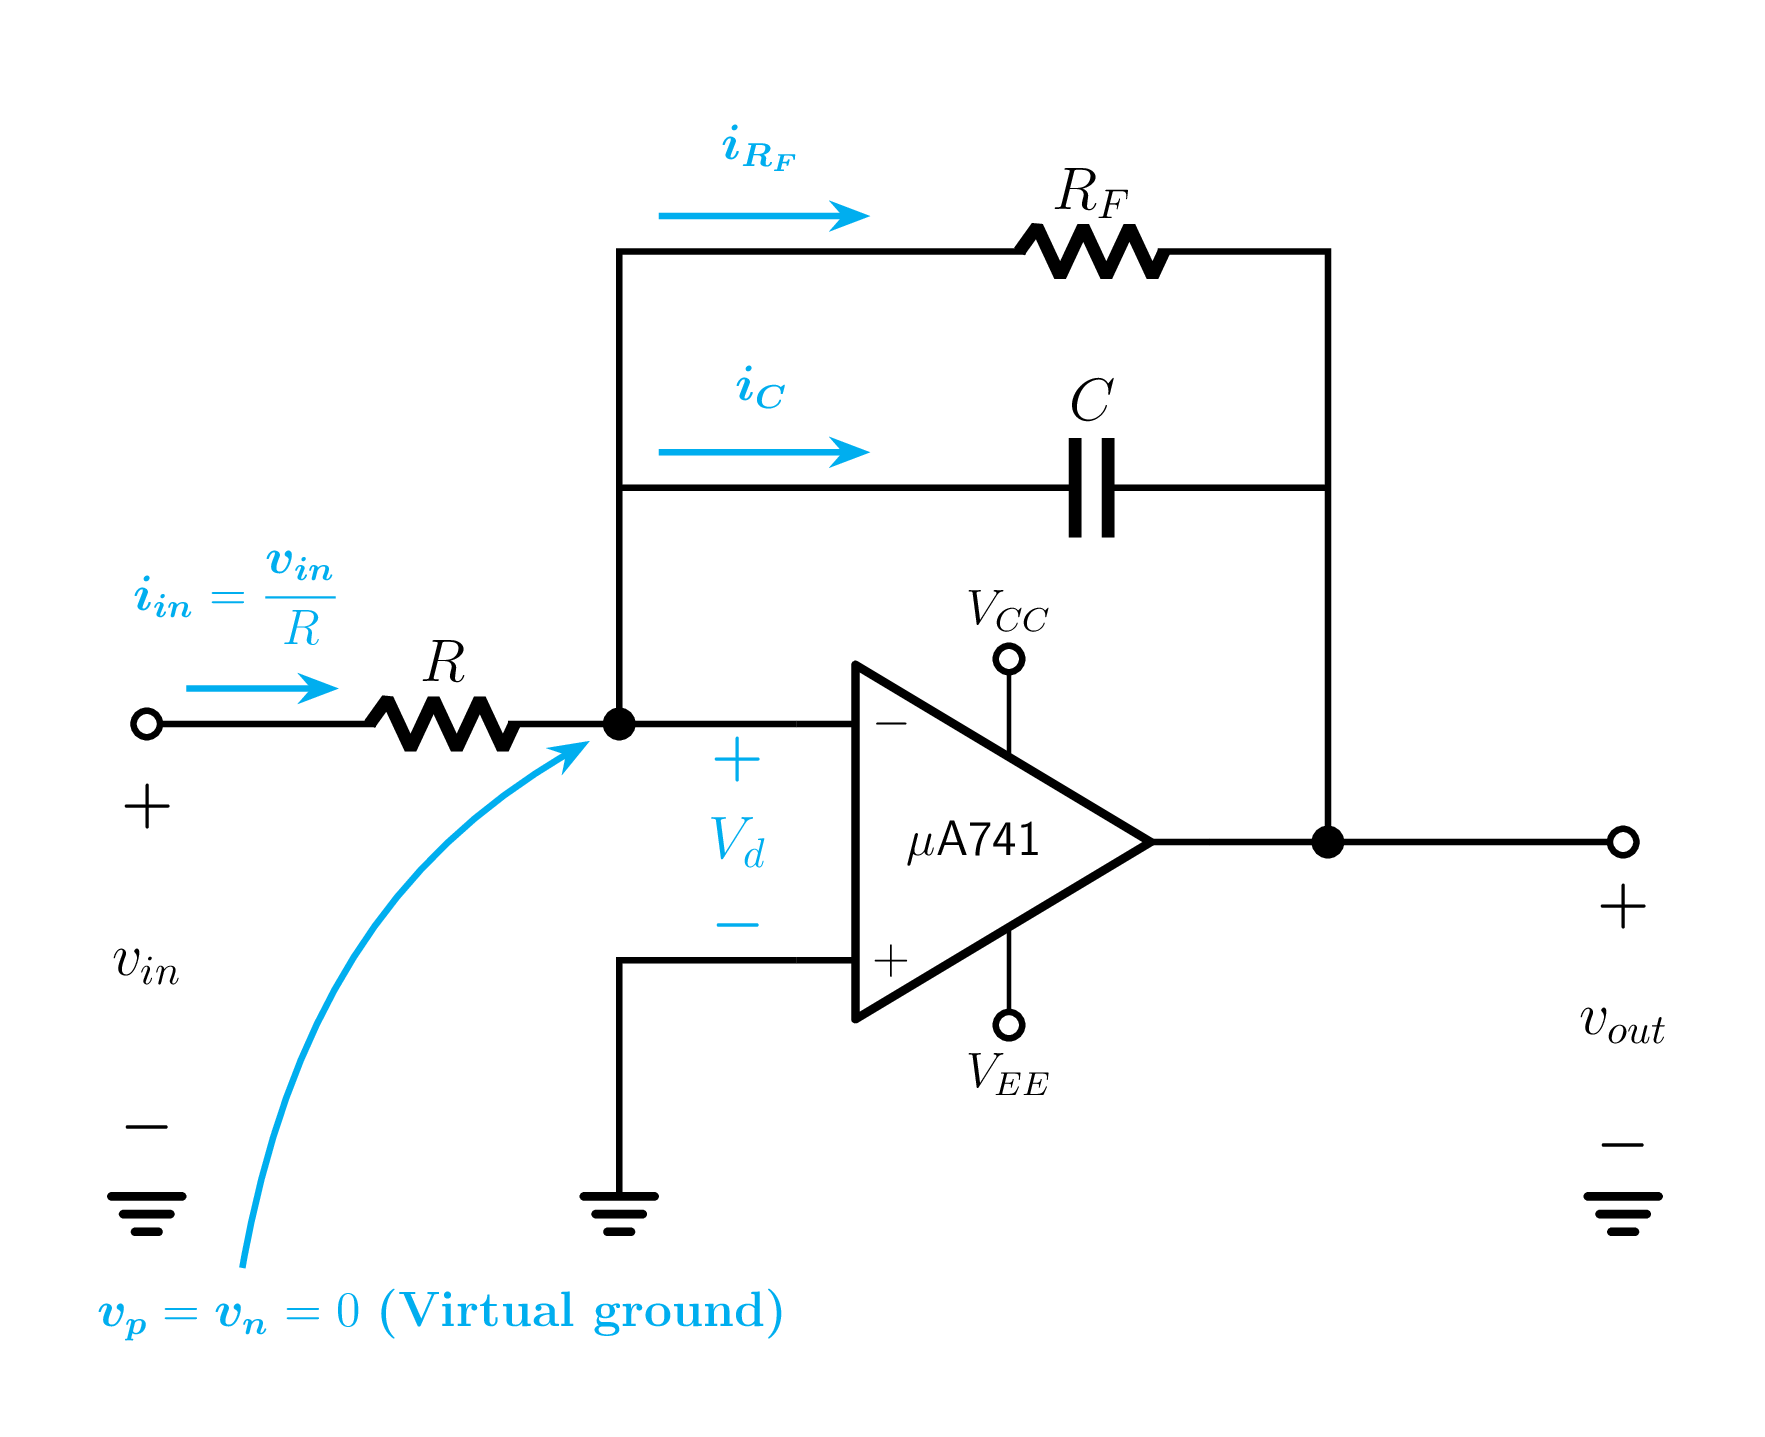
\includegraphics[scale=0.23]{images/practical_integrator.png}
      \caption{Practical integrator circuit}
      \label{fig:theoretical_practical_integrator}
    \end{figure}

    The resulting circuit is an inverting amplifier with $R_F||\cfrac{1}{Cs}$ acting as the feedback resistance.
    The gain of such an amplifier is given by:
    \begin{align*}
      \cfrac{V_{out}(s)}{V_{in}(s)} &= - \cfrac{R_F||\cfrac{1}{Cs}}{R}\\
      &= - \cfrac{R_F}{R} \cfrac{1}{(1 + R_F Cs)}
    \end{align*}

    Thus, the frequency response of the practical integrator is given by,
    \begin{align}
      H(s) &= \frac{-R_{F} || \frac{1}{Cs}}{R} \\
      H(j\omega) &= \frac{-R_{F}}{R} \left[ \frac{1}{1+R_{F}Cj\omega} \right] \label{eq:freq_response}
    \end{align}

    The magnitude and phase response are given by,
    \begin{align*}
    |H(j\omega)| &= \cfrac{R_{F}}{R}\cfrac{1}{\sqrt{1+\omega^{2}R_{F}^{2}C^{2}}} \\
    \angle H(j\omega) &= \pi - tan^{-1}(\omega R_{F}C)
    \end{align*}

    \underline{DC gain} is obtained by putting $\omega = 0$ in equation \ref{eq:freq_response}.
    \begin{equation}
      \text{DC gain} = H(j0) = -\frac{R_f}{R} \equiv -20\log_{10}(\cfrac{R_F}{R}) \text{ dB}
    \end{equation}

    \underline{Phase shift} $\Delta\phi$ between the input and output signals is given by
    \begin{equation}\label{eq:phase_shift}
      \Delta\phi = \pi - \tan^{-1}(\omega R_FC)
    \end{equation}

    The practical integrator acts as a first order filter with corner frequency (also cut-off or pole frequency) at $f = -1/R_FC$.
    Thus, \underline{$f_{-3dB}$} or \underline{cutoff-frequency} is given by
    \begin{equation}\label{eq:f3db}
      f_{-3dB} = \frac{1}{2\pi R_FC}
    \end{equation}

    \underline{Unity gain bandwidth} $\omega_u$ is obtained from $|H(j\omega)| = 1$:
    \begin{align*}
      H(j\omega) = 1 &= \cfrac{R_{F}}{R}\cfrac{1}{\sqrt{1+\omega^{2}R_{F}^{2}C^{2}}} \\
      \left(\cfrac{R_F}{R}\right)^2 &= 1 + (\omega R_FC)^2 \\
      \left(\cfrac{R_F}{R}\right)^2 &\approx (\omega R_FC)^2 & \left(\text{for } \cfrac{R_F}{R} \gg 1\right)\\
      \implies \omega_u &= \cfrac{1}{RC} \text{ or } f_u = \cfrac{1}{2\pi RC}\numberthis \label{eq:unity_gain_bw}
    \end{align*}

    \underline{Roll-off rate} of the frequency response is theoretically -20 dB/decade.

  \newpage
  \section{Design}
    % TODO Stepwise design
    Q. Design a $\mu$A741 based voltage integrator with unity gain and
    $f_{-3dB} = f_{in}/15$ for a sinusoidal input
    $v_{in} = 2 sin(4000\pi t)$, keeping the phase error below 5\%.
    \begin{align*}
        \text{Let C} \! &=0.01\mu F , \\
        f_{in} &=2000 Hz\\
        f_{-3dB} &=\frac{f_{in}}{15} = 133.33 Hz \\
        \frac{1}{2\pi R_{F}C} &= 133.33\\
        \frac{1}{2\pi RC} &= 2000\\
        R &=7.96k\Omega\\
        R_{F} &=119.37k\Omega\\
    \end{align*}

  \newpage
  \section{Simulation}
    % TODO Add captions
    % TODO Arrange
    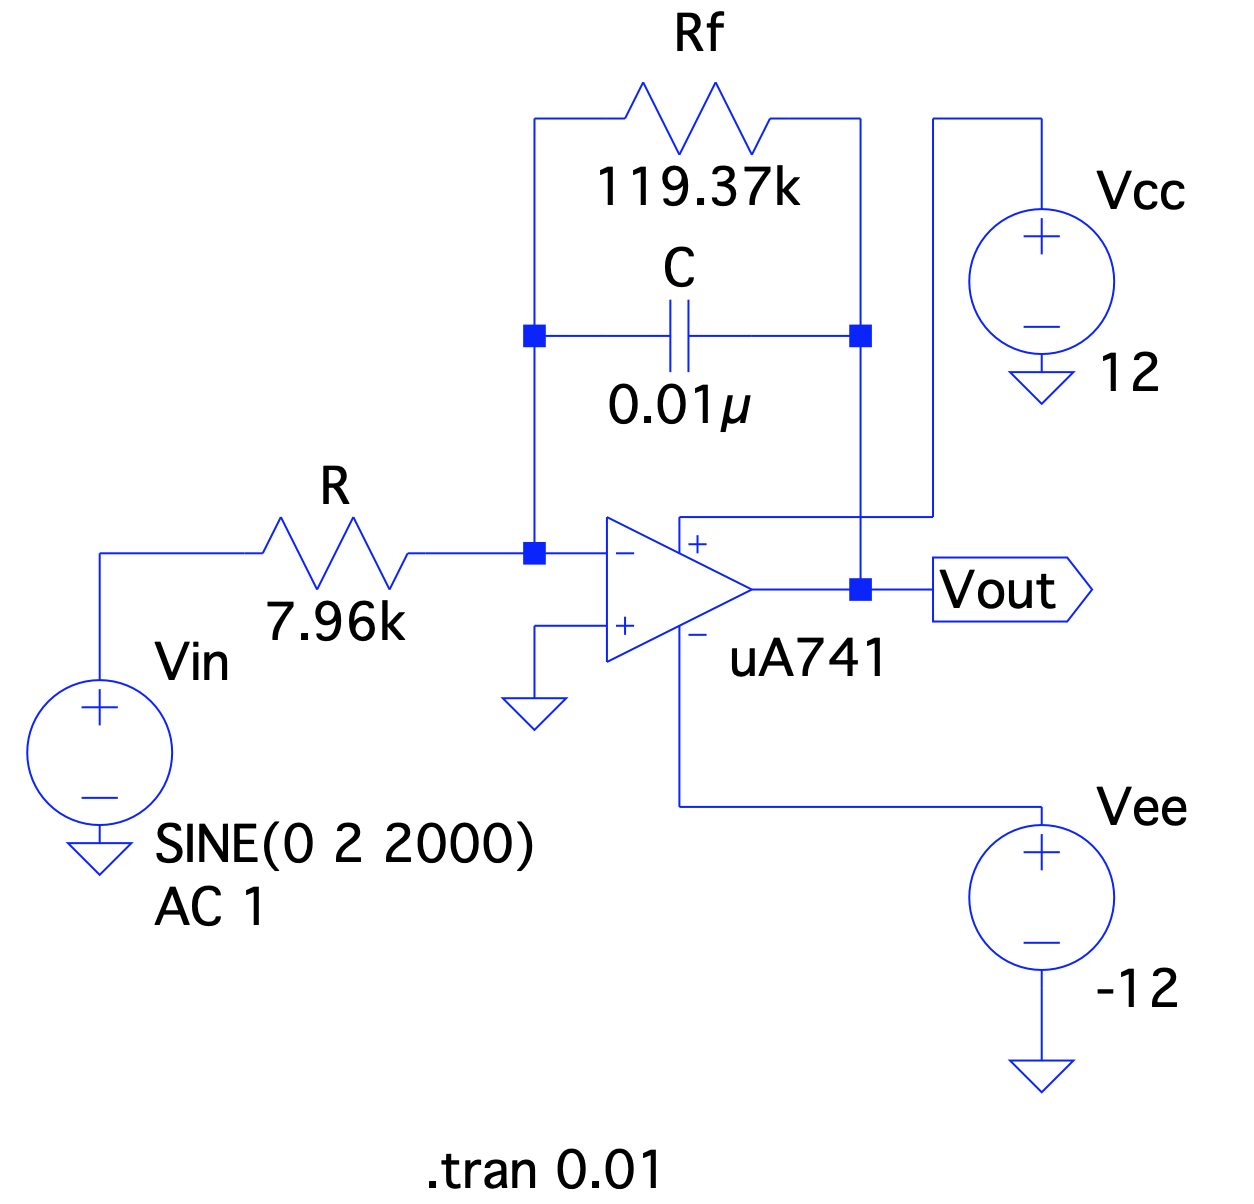
\includegraphics[scale=0.25]{sim_circuit}\\
    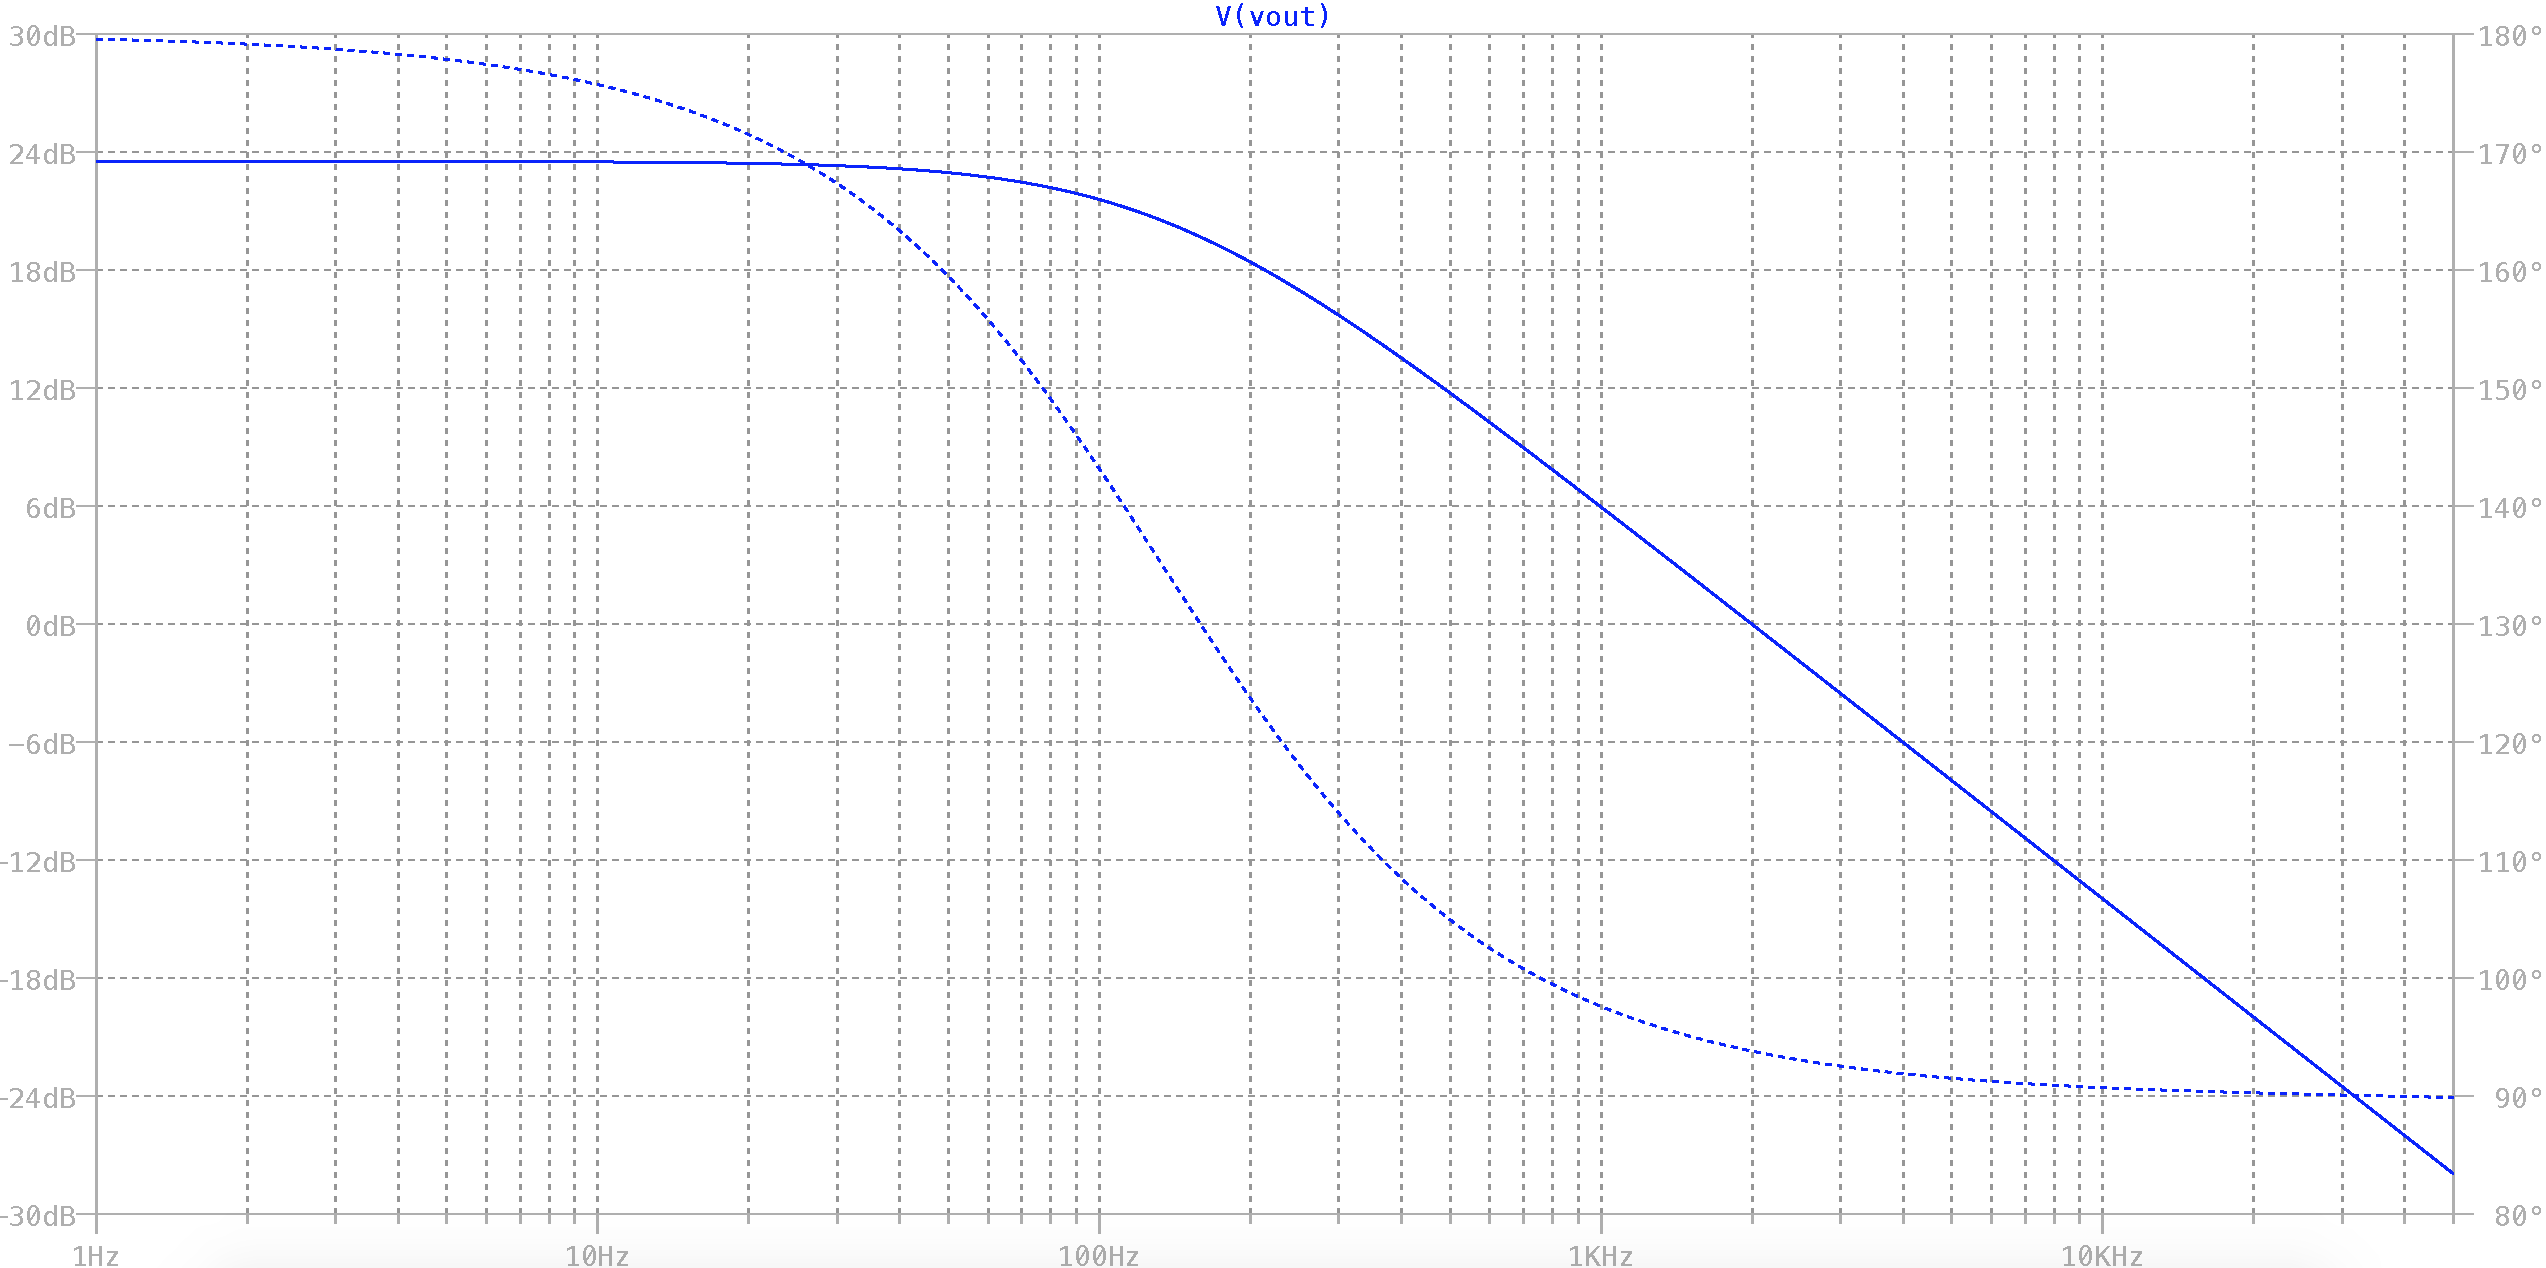
\includegraphics[scale=0.25]{sim_plot_fd}\\
    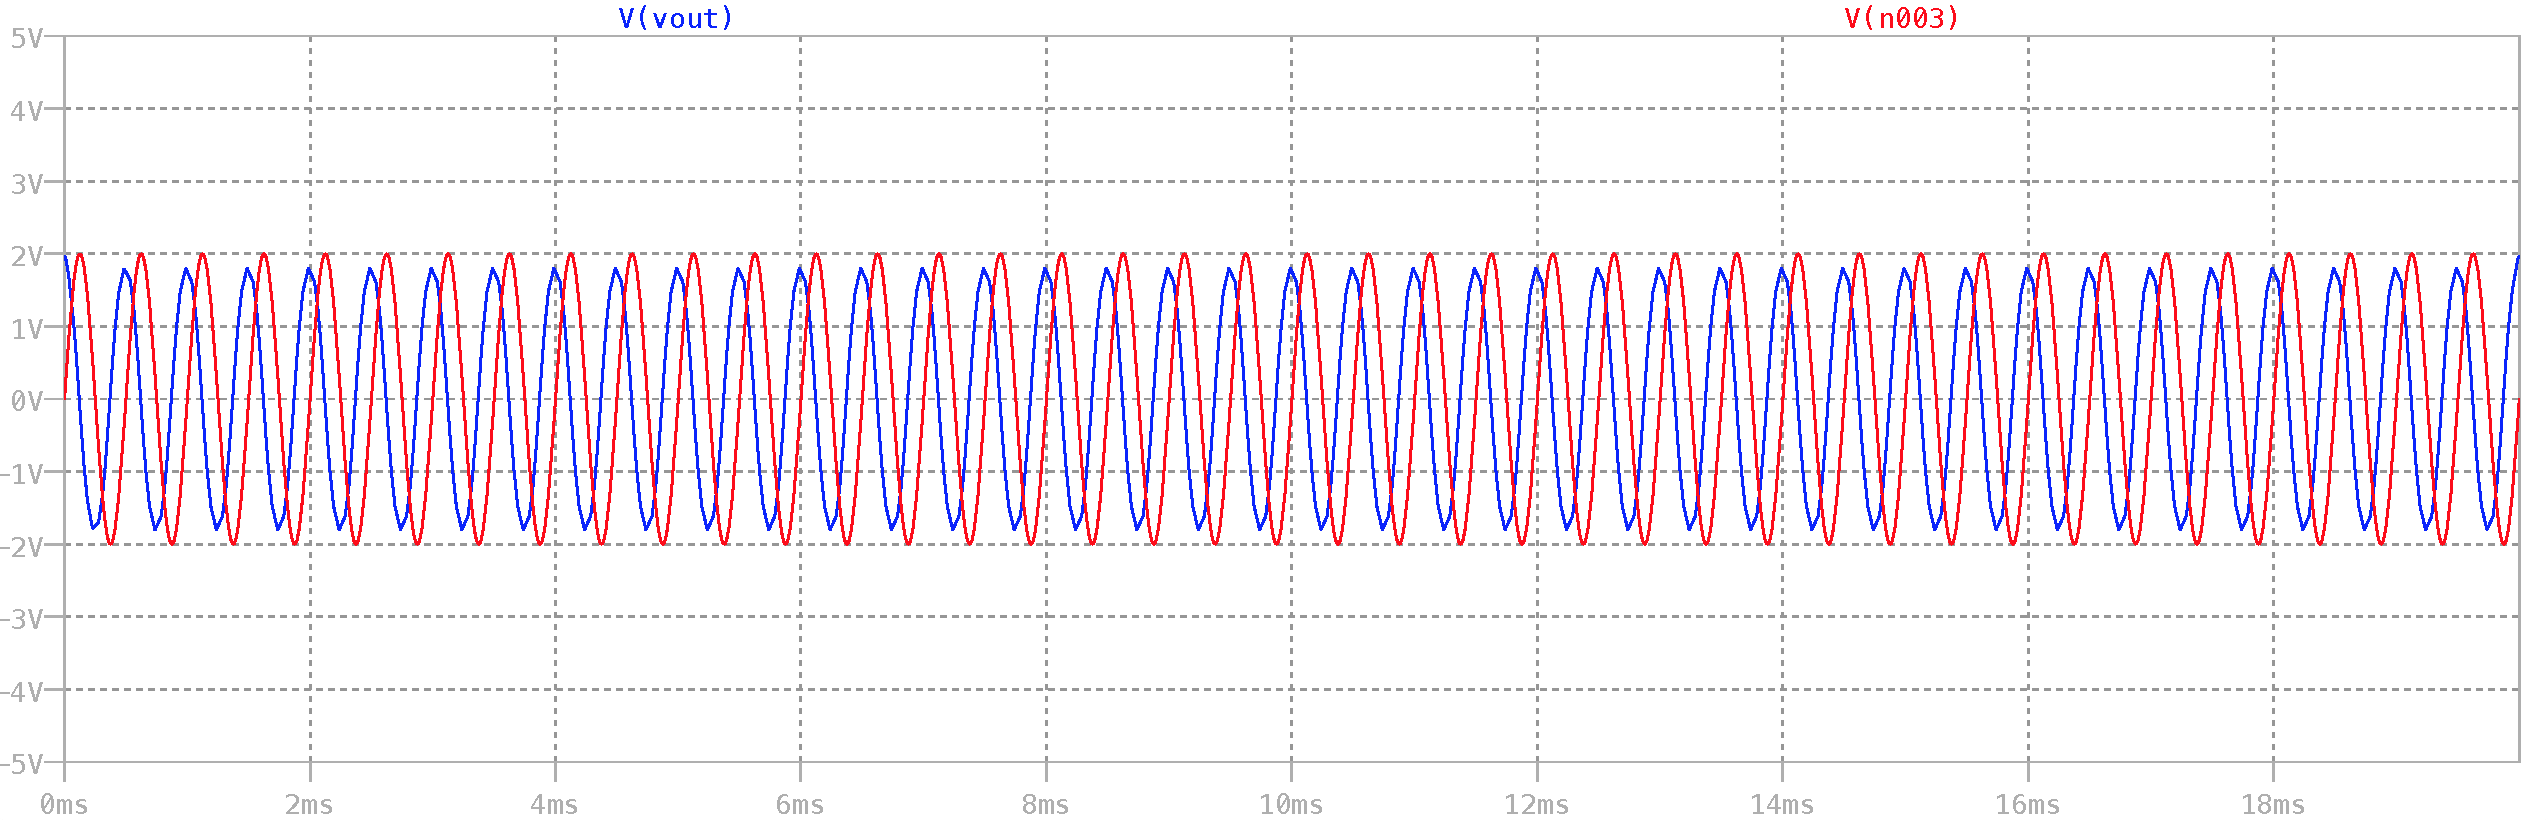
\includegraphics[scale=0.25]{sim_plot_td}


  \newpage
  \section{Waveforms}
    % TODO Add captions and labels
    % TODO Merge with observations
    % TODO Arrange
    \includegraphics[scale=0.25]{results_q1}\\
    \includegraphics[scale=0.25]{results_q3}\\
    \includegraphics[scale=0.25]{results_q4_2}


  \newpage
  \section{Observations}
    %===A===
    \textbf{A}. The practical integrator is first designed based on the following constraints:
    Unity gain, $f_{-3dB} = f_{in}/15$ for a sinusoidal input
    $v_{in} = 2 sin(4000\pi t)$ and a phase error below 5\%.

    A leading phase sinusoidal wave appears at the output of the integrator as shown in figure \ref{fig:results_q1}.
    The DC gain, -3dB frequency $f_{3dB}$, unity gain frequency $f_u$, roll-off rate and phase shift are noted from the waveforms obtained on the DSO and the phase error is verified to be below 5\%.

    \begin{figure}
      \includegraphics[scale=0.25]{images/results_q1.jpeg}
      \caption{Result of passing a sinusoidal input through the integrator; \color{cyan}$V_{out}$ \color{black}\& \color{orange}$V_{in}$}
      \label{fig:results_q1}
    \end{figure}

    % TODO Show calculations
    \begin{itemize}
      \item[] DC gain = 14.89
      \item[] -3dB frequency $f_{-3dB}$ = 132 Hz
      \item[] Unity gain frequency $f_u$ = 2.07 kHz
      \item[] Roll-off rate = -18.35 dB/decade
      \item[] Phase shift $\phi$ = $1.608^{c}$ or $92.13^{\circ}$, an error of 2.4\%
    \end{itemize}

    %===B===
    \textbf{B}. The feedback resistor $R_F$ is then removed and the effect on the op-amp integrator configuration is observed.

    \begin{figure}
      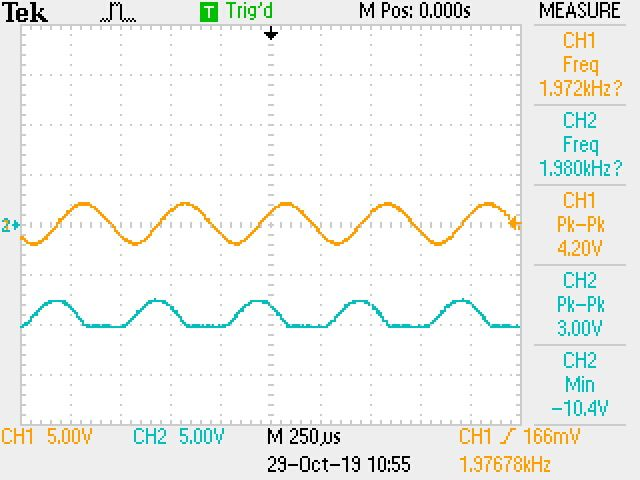
\includegraphics[scale=0.25]{images/results_q2.jpeg}
      \caption{The output of the integrator circuit without $R_F$}
      \label{fig:results_q2}
    \end{figure}

    The output is given by $V_{out}=\pm V_{sat}$ due to the capacitor acting as an open circuit at low frequencies as shown in figure \ref{fig:results_q2}.This sends the op-amp into an open loop configuraton.

    %===C===
    \textbf{C}. The sinusoidal input is replaced by a square wave of 4$V_{pk-pk}$ amplitude and a frequency of 2kHz to observe the integration operation of the configuration more clearly.

    \begin{figure}
      \includegraphics[scale=0.25]{images/results_q3.jpeg}
      \caption{Result of integrating a square wave \color{cyan}$V_{out}$ \color{black}\& \color{orange}$V_{in}$}
      \label{fig:results_q3}
    \end{figure}

    A triangular waveform is obtained as a result of the square wave being integrated, as shown in figure \ref{fig:results_q3}.

    $C\Delta V=I\Delta t$\\
    Substituting $C=0.01\mu F$, $I=\frac{2}{8k}$, $\Delta t=\frac{0.5}{2000}$, \\
    $\Delta V = 6.25 V$\\
    The output triangular waveform has a peak to peak voltage of around 6.25 V.

    D. The frequency of the input is lowered to 130Hz and the output is observed again on the DSO.

    \begin{figure}
      \includegraphics[scale=0.25]{images/results_q4_2.jpeg}
      \caption{Effect of lowering the input frequency on the output \color{cyan}$V_{out}$ \color{black}\& \color{orange}$V_{in}$}
      \label{fig:results_q4}
    \end{figure}

    $C\Delta V=I\Delta t$\\
    Substituting $C=0.01\mu F$, $I=\frac{2}{8k}$, $\Delta t=\frac{0.5}{130}$, \\
    $\Delta V = 96.15 V$ \\
    Since $\Delta V > 2V_{sat}$, $V_{out}$ gets clipped as shown in figure \ref{fig:results_q4}.


  \newpage
  \section{Results \& Conclusions}
    % TODO Add more results and better conclusions
    The $\mu$A741 based voltage integrator was designed and implemented successfully.
\end{document}
